\documentclass{article}
\usepackage{graphicx}
\usepackage{float}
\usepackage{subcaption}
\usepackage{hyperref}
\hypersetup{
	colorlinks=true,
	linkcolor=blue,
	citecolor=blue,
	filecolor=magenta,
	urlcolor=black        
}
\usepackage[a4paper,top=2cm,bottom=2cm,left=3cm,right=3cm,marginparwidth=1.75cm]{geometry}
\usepackage[T1]{fontenc}
\usepackage[polish]{babel}
\usepackage{csquotes}
\usepackage[sorting=none, language=polish]{biblatex}


\addbibresource{bibliography.bib}

\title{Rozwój aplikacji do analizy danych w eksperymencie WarsawTPC -- raport}
\author{Maciej Bajor \\ Przemysław Szyc \\ Szymon Sławiński \\\\ Opiekun: dr hab. Artur Kalinowski}

\begin{document}

\maketitle

\section{Wstęp}
% MB
Analiza danych w eksperymencie WarsawTPC~\cite{WAWTPC}, zajmującym się badaniem zjawiska\linebreak fotodezintegracji atomów tlenu i węgla, odbywała się do tej pory przy pomocy programów z repozytorium TPCReco~\cite{TPCReco}, napisanych w języku C++. Istotnym elementem tego oprogramowania, kluczowym przy dostrajaniu narzędzi do analizy, są symulacje zdarzeń metodą Monte Carlo.

W celu poprawy jakości automatycznej analizy danych z eksperymentu stworzono w 2023 roku zestaw programów napisanych w języku Python, umożliwiających rekonstrukcję i analizę zdarzeń z wykorzystaniem uczenia maszynowego.
% /MB

\section{Cel projektu zespołowego}
% MB
Założenia projektu skupiały się na poprawie działania rekonstrukcji torów z użyciem uczenia maszynowego. Do tego celu potrzebne było przygotowanie odpowiednich danych wejściowych z symulacji, które odpowiadałyby danym z eksperymentu - stąd zaszła konieczność wykonania porównań, a także poprawek w kodzie do symulacji, aby uzyskać jak najlepszą zgodność z danymi doświadczalnymi.

Zadania w obszarze uczenia maszynowego obejmowały optymalizację formatu danych wejściowych z punktu widzenia przepustowości, a więc przyspieszenie odczytywania danych z plików w formacie \texttt{.ROOT}~\cite{root}, trening modelu rozpoznającego punkty krańcowe torów, test wydajności modelu i porównanie z obecnym algorytmem na danych symulowanych i rzeczywistych. W dalszej przyszłości powinna nastąpić integracja modelu ze środowiskiem TPCReco z użyciem API do C++  z pakietu TensorFlow~\cite{TensorFlow}.
% /MB
\section{Repozytoria i obszary robocze projektu}
% MB
Zmiany w kodzie wprowadzane były w dwóch repozytoriach w serwisie GitHub~\cite{GitHub} - odgałęzieniu głównego repozytorium TPCReco~\cite{TPCRecofork}, oraz w plikach repozytorium MachineLearning~\cite{WAWTPCfork}, odpowiedzialnych za trening i sprawdzanie dokładności modeli uczenia maszynowego. Zaakceptowane zmiany w kodzie trafiały do gałęzi poprzedzonych przedrostkiem ZPS.

Oprócz powyższych, zespół korzystał z przestrzeni w Notion~\cite{Notion} na potrzeby związane z tworzeniem i podziałem zadań, przekazywaniem raportów cząstkowych opiekunowi projektu, oraz spisywaniem instrukcji do niektórych czynności. 

Komunikacja w zespole odbywała się na czacie w Google Workspace oraz na spotkaniach z opiekunem, organizowanych co dwa tygodnie. Wymiana plików miała miejsce za pomocą folderu współdzielonego na Dysku Google.

Zadania wymagające mocy obliczeniowej wykonywano początkowo w Google Colab~\cite{Colab} i lokalnie, następnie na komputerze wydziałowym bez koprocesora graficznego, a pod koniec uzyskano dostęp do maszyn HPC ICM~\cite{ICM}.
% /MB

\section{Symulacje Monte Carlo}
% MB
Działania w zakresie symulacji zdarzeń skupiały się na zapewnieniu potrzebnych zbiorów treningowych i walidacyjnych do uczenia maszynowego, a także na porównaniu zgodności przebiegu torów z rzeczywistymi danymi.
\ 
Wprowadzono do kodu \texttt{TPCDigitizerRandom} prostą poprawkę, pozwalającą na ustalanie rozmycia torów w rozkładzie płaskim efektywnej dyfuzji; minimalne i maksymalne wartości sigm można podać w pliku konfiguracyjnym Monte Carlo w następujący sposób:

\begin{verbatim}
"TPCDigitizerRandom": {
      "sigmaXYmin": 0.75,
      "sigmaXYmax": 1.5,
      "sigmaZmin": 0.75,
      "sigmaZmax": 1.5,
      "NSamplesPerHit": 100,
      "MeVToChargeScale": 100000
    }
\end{verbatim}
 
Wykonano także porównania symulacji z danymi rzeczywistymi, z wykorzystaniem dopasowań z GUI. Przy ustalonym wierzchołku generowano tory zgodnie z parametrami dopasowań i energią wiązki. Wykonane porównania wskazują na rozbieżności w szczególnych przypadkach, głównie gdy produkty reakcji poruszały się wzdłuż którejś z osi detektora (przykładowe zdarzenie znajduje się na Rysunku~\ref{fig:porownanie}). Na potrzeby wykonania porównań również wprowadzono poprawki w kodzie, między innymi zaimplementowano możliwość ustalania granic osi w funkcji \textit{plf.plotEvent} z repozytorium MachineLearning~\cite{WAWTPCfork}, a także przygotowano do wprowadzenia zmiany w modułach symulacji \texttt{ReactionTwoProng} i \texttt{EventGenerator} z repozytorium TPCReco~\cite{TPCRecofork}, które wymagają jeszcze konsultacji z autorem oryginalnego kodu.

\begin{figure}[htbp]
    \centering
    \begin{subfigure}[b]{\textwidth}
        \centering
         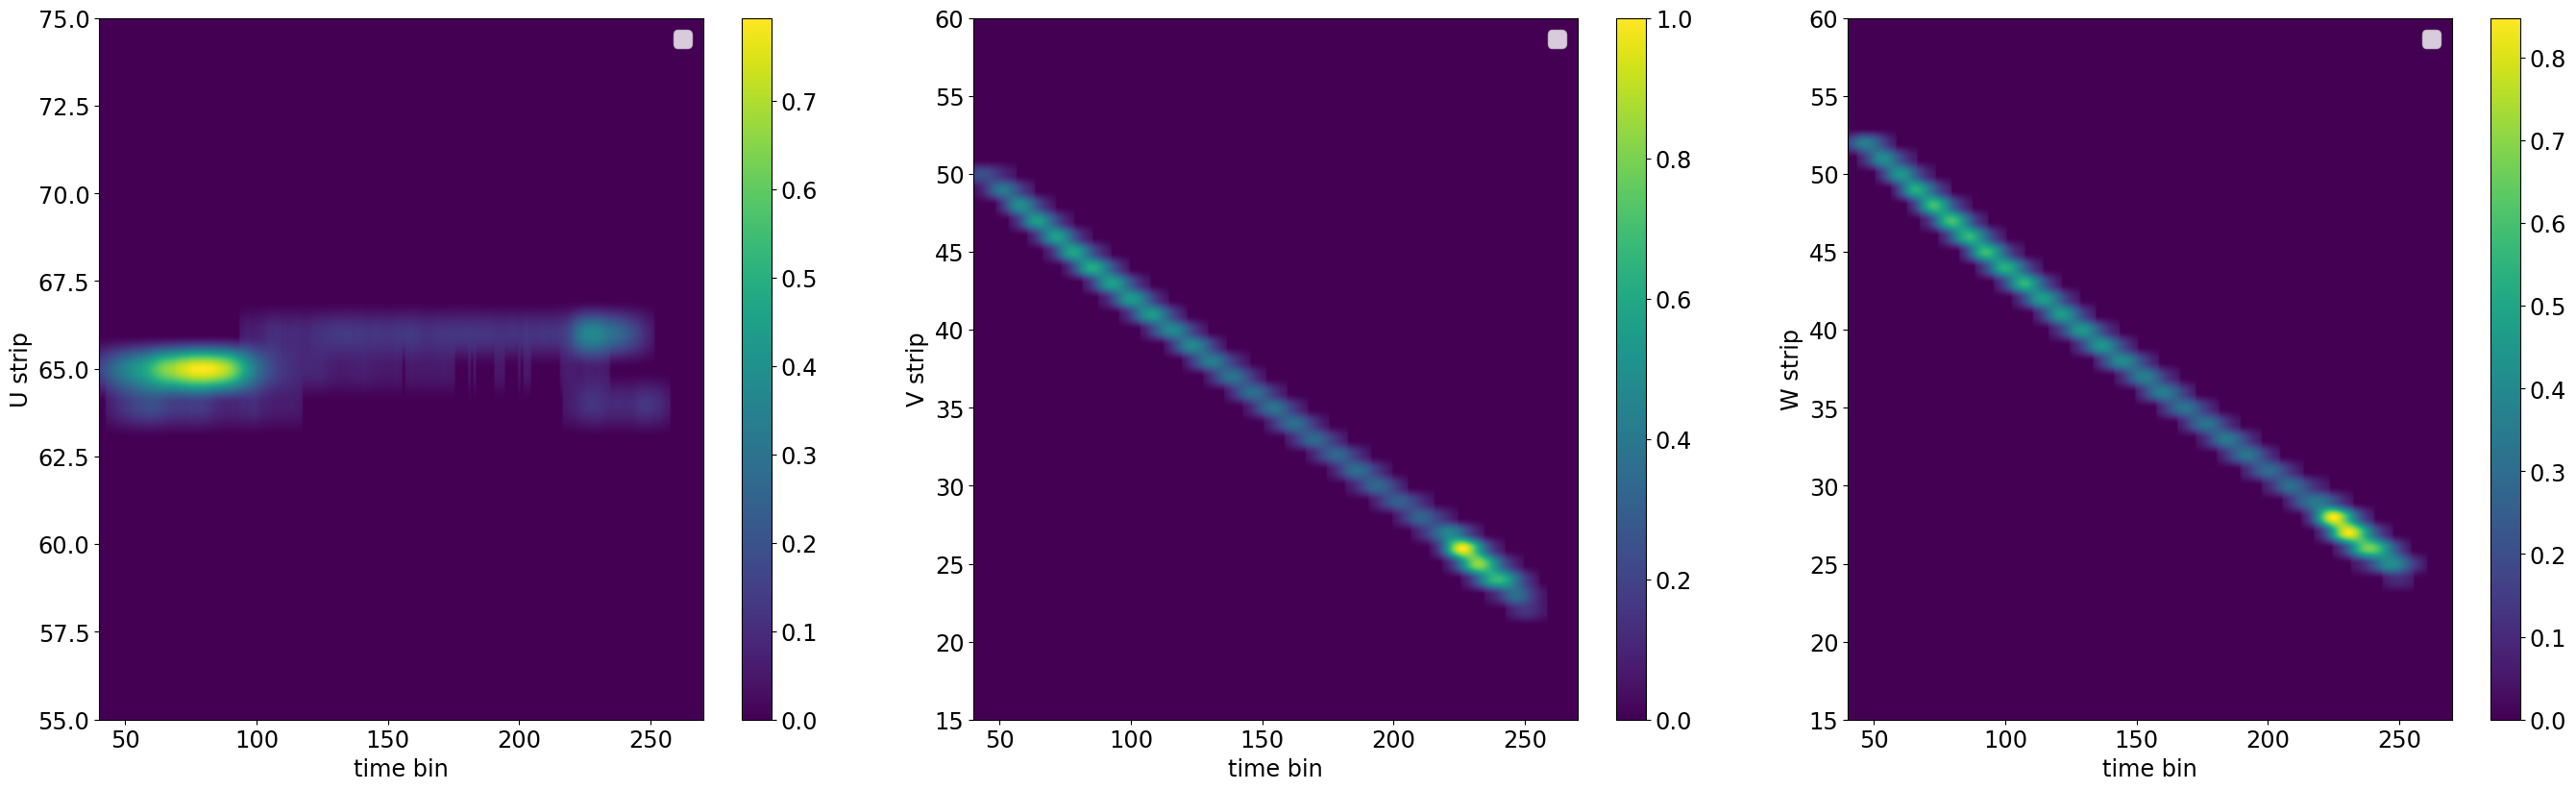
\includegraphics[width=\textwidth, trim={0cm 0cm 0cm 0cm},clip]{img/event1014_real.png}
         \caption{Zdarzenie nr 1014 z porcji danych eksperymentalnych.}
         \label{fig:real}
    \end{subfigure}
    \begin{subfigure}[b]{\textwidth}
         \centering
         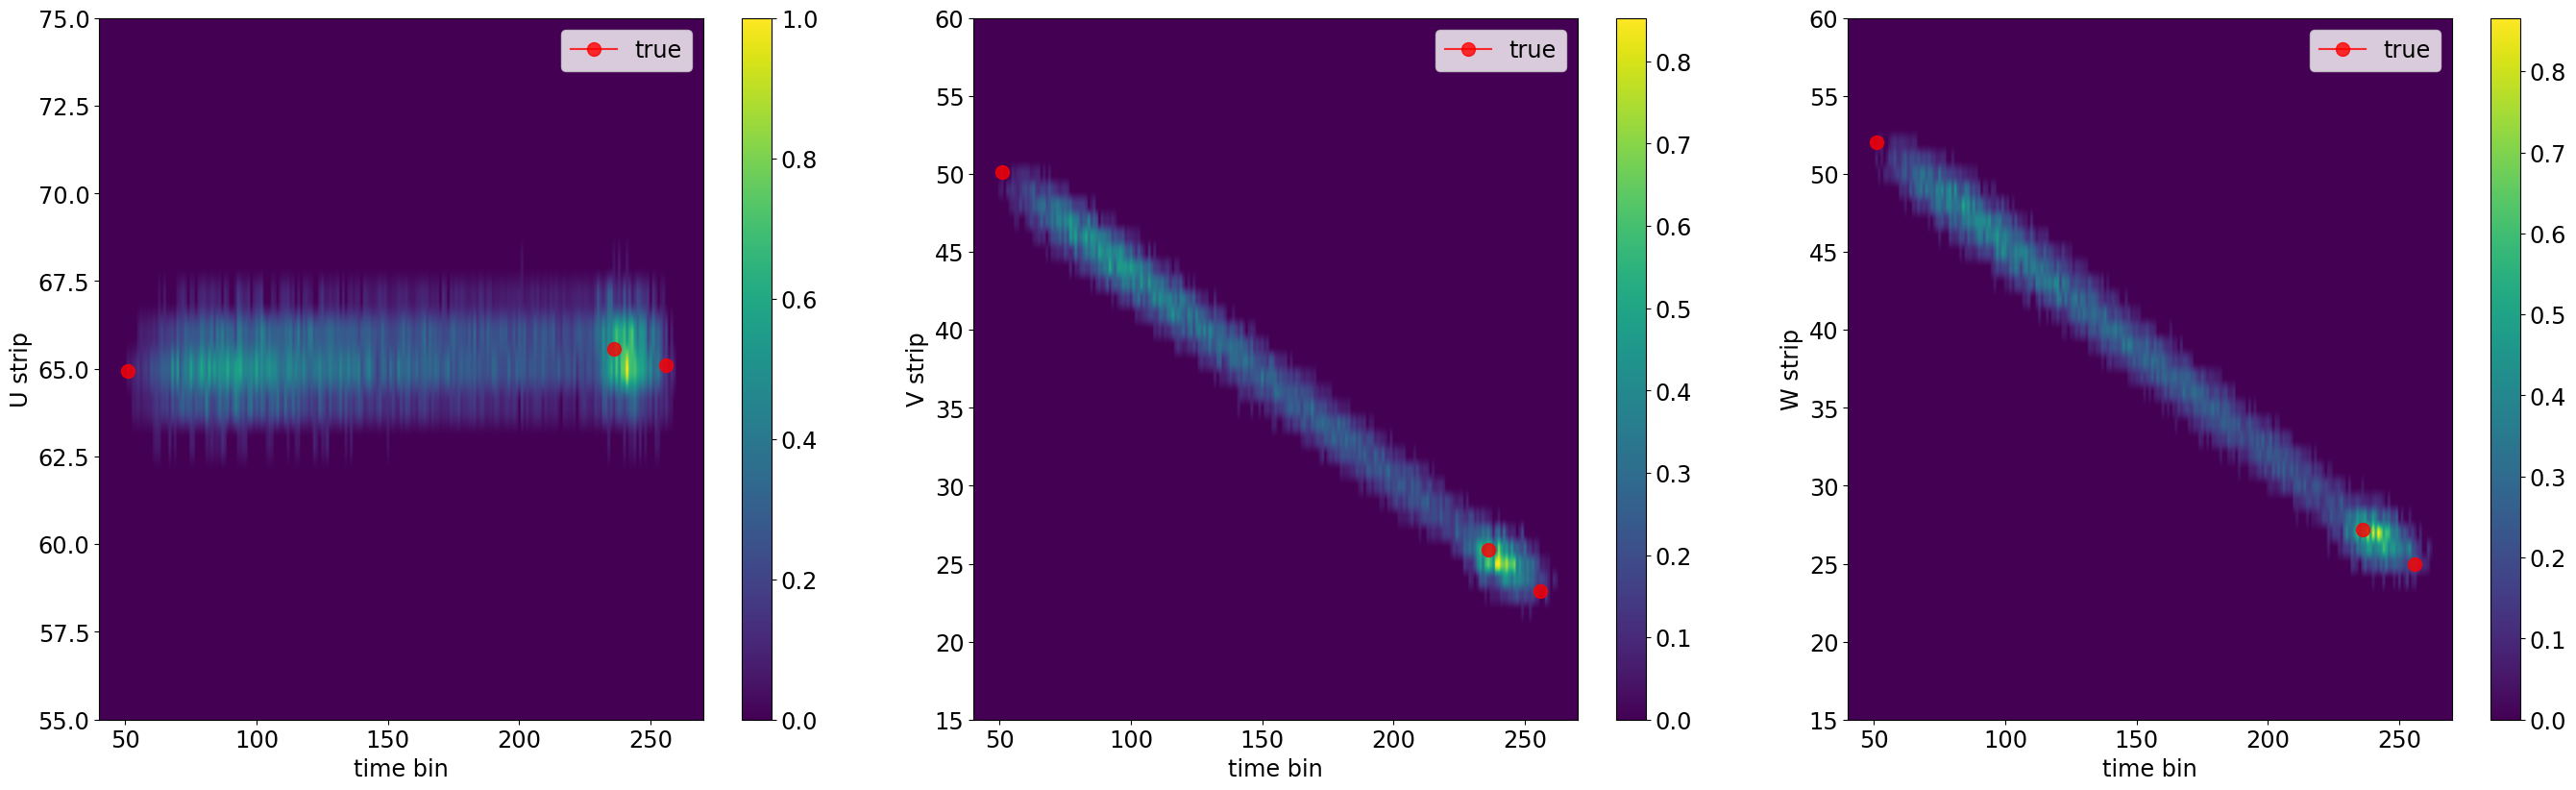
\includegraphics[width=\textwidth, trim={0cm 0cm 0cm 0cm},clip]{img/event1014_sim_1_5.png}
         \caption{Zdarzenie symulowane z wykorzystaniem \texttt{TPCDigitizerRandom} z wprowadzoną poprawką (efektywna dyfuzja 1,5 mm).}
         \label{fig:sim1}
    \end{subfigure}
    \begin{subfigure}[b]{\textwidth}
         \centering
         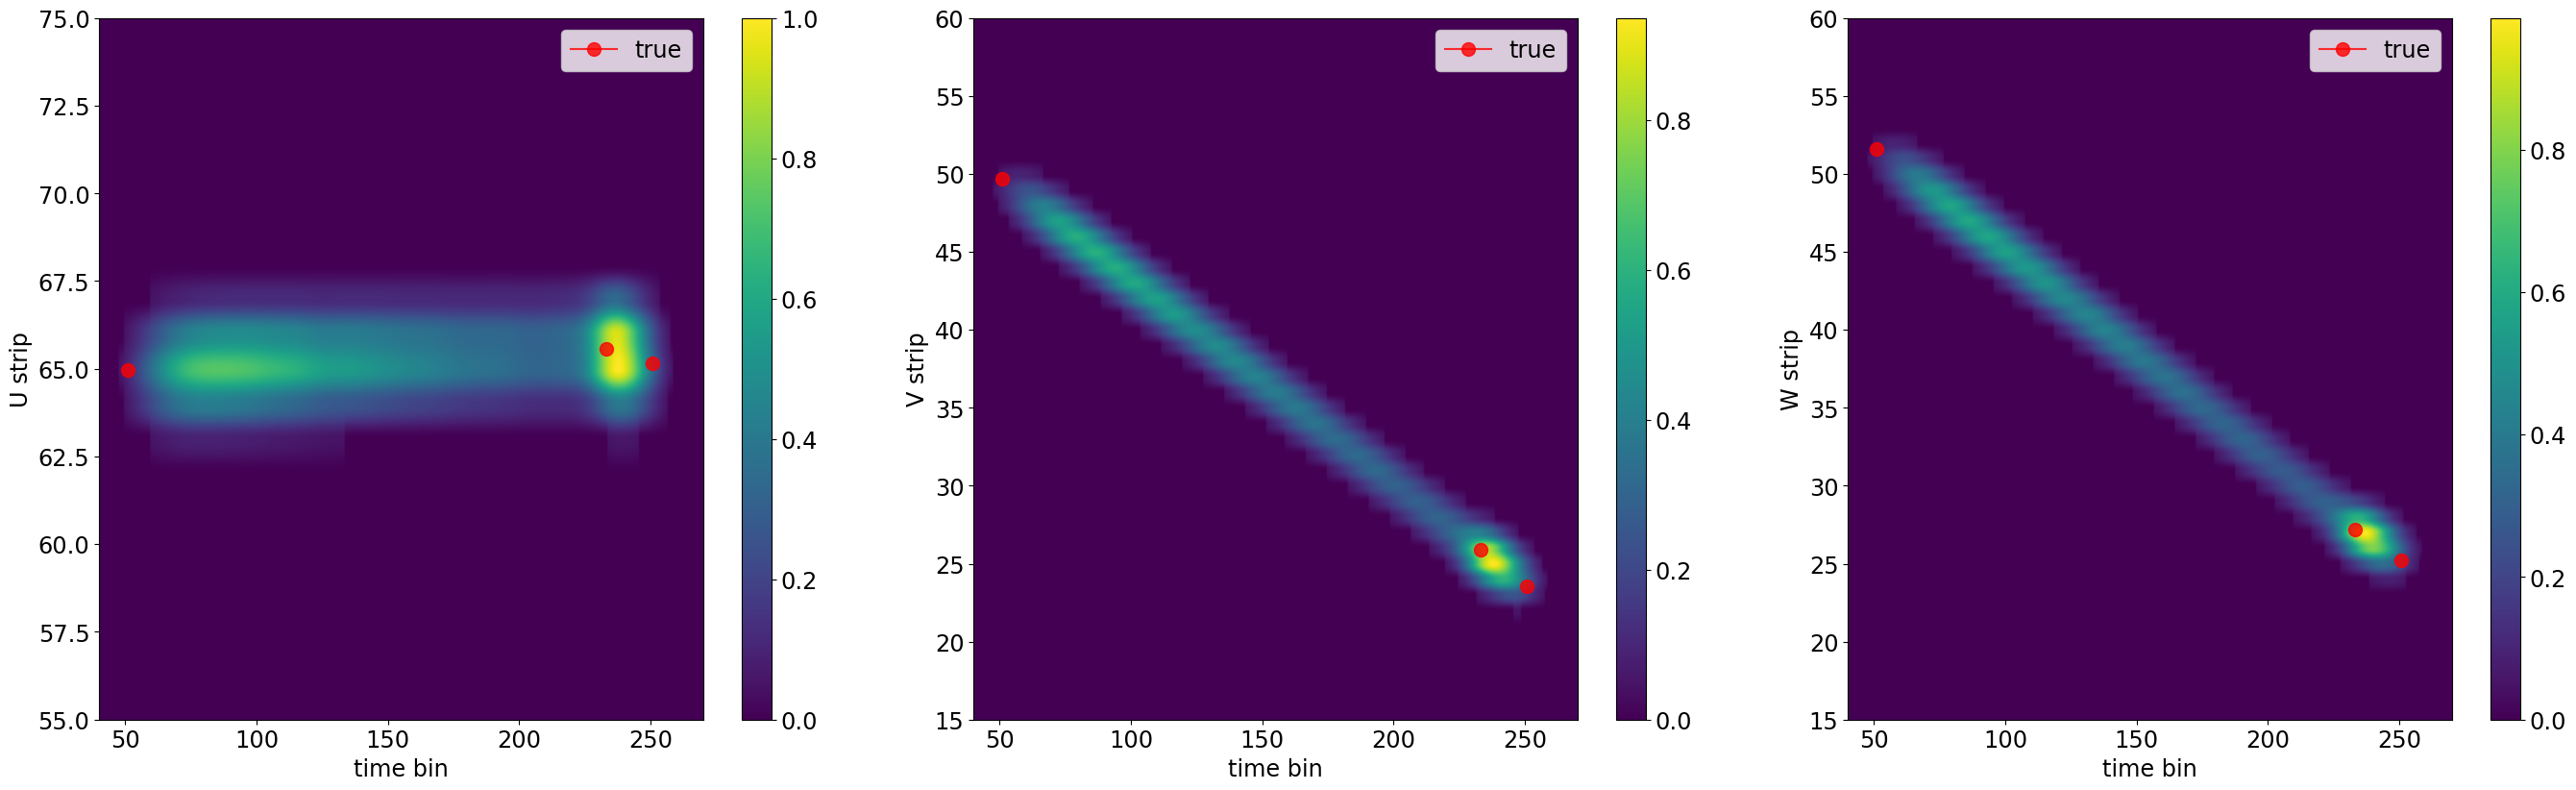
\includegraphics[width=\textwidth, trim={0cm 0cm 0cm 0cm},clip]{img/event1014_simSRC.png}
         \caption{Zdarzenie symulowane z użyciem \texttt{TPCDigitizerSRC} (efektywna dyfuzja 1,5 mm).}
         \label{fig:sim2}
    \end{subfigure}
    \caption{Porównanie zdarzenia odczytanego z danych eksperymentalnych dla energii wiązki $E=11,5$ MeV ze zdarzeniami symulowanymi na bazie dopasowania z GUI (czerwone punkty to położenia wierzchołka i końców torów wyznaczone na bazie dopasowania).}
    \label{fig:porownanie}
\end{figure}
 
W odniesieniu do generowania danych, korzystania z GUI i rekonstrukcji zdarzeń, stworzono instrukcje w Notion~\cite{NotionDocs} w ramach ulepszania dokumentacji, aby łatwiej było zaznajomić się z narzędziami pakietu TPCReco.
% /MB

\section{Uczenie Maszynowe}
% By Przemysław Szyc - wersja 1.0
Rekonstrukcji położenia torów cząstek można dokonywać w formacie docelowym, czyli we współrzędnych XYZ,
oraz dla każdej projekcji oddzielnie, w układzie odniesienia UVWT~\cite{UVWT}.

W przypadku formatu docelowego XYZ model, którego danymi wejściowymi są tablice o wymiarach (256, 512, 3) - (numer paska, numer przedzialu czasowego, numer rzutu) - reprezentujące odczyty z detektorów, dokonuje rekonstrukcji położeń trzech punktów w kartezjańskim układzie współrzędnych, tzn. przestrzeń wyjść składa się z trzech wektorów 3-wymiarowych.

Rekonstrukcja w formacie UVWT polega na tym, że dla każdej podprzestrzeni (UT, WT, VT) rekonstrukcja wykonywana jest niezależnie. Wektorem wejściowym są tablice (256, 512, 1), a wyjściem współrzędne rzutów punktów na daną podprzestrzeń (dwa wektory 3-elementowe). Rekonstrukcja ta wymaga też użycia funkcji mapującej wektory z przestrzeni UT, VT, WT do przestrzeni XYZ po dokonaniu rekonstrukcji.\\\\
Podczas projektu oba te podejścia były rozwijane:
\subsection{Rekonstrukcja we współrzędnych XYZ}
W kontekście tej metody wykonano następujące zadania:
\begin{enumerate}
    \item Umożliwiono konwersję danych z formatu .root do formatu .tfrecord;
    \item Stworzono notatnik~\cite{ColabML}, w którym możliwym jest trenowanie modelu w środowisku Google Colab.
\end{enumerate}
Konwersja danych odbywa się w notatniku \href{https://github.com/mwbaj/MachineLearning/blob/ZPS_2023_winter/WAWTPC/ROOT_to_TFRecord.ipynb}{\texttt{ROOT\_to\_TFRecord.ipynb}}, za konwersję odpowiedzialna jest funkcja \textit{process\_and\_save}.
Format danych wyjściowch (target w zmiennych XYZ czy UVWT) wybierany jest poprzez podanie odopwiedniego argumentu do funkcji \textit{process\_and\_save}.

Praca w środowiku Google Colab została umożliwiona poprzez dodanie gałęzi \href{https://github.com/mwbaj/MachineLearning/tree/ZPS_colab-friendly}{\textit{ZPS\_colab-friendly}} i stworzenie wersji notatników zintegrowanych z tym środowiskiem oraz Dyskiem Google. 
\subsection{Rekonstrukcja w współrzędnych UVWT}
Wykonane zadania w celu rozwijania tej metody:
\begin{enumerate}
    \item Do algorytmu zmiany formatu danych z .root do .tfrecord dodano możliwość konwersji zmiennej target do współrzędnych UVWT;
    \item Przygotowano modele ResNet-50~\cite{ResNet} oraz początkowy model konwolucyjny (schemat na Rysunku~\ref{fig:schemat}) do treningu w tym formacie;
    \item Zintegrowano funkcje do wizualizacji danych z działaniem tych modeli.
\end{enumerate}
W notatniku \href{https://github.com/mwbaj/MachineLearning/blob/ZPS_2023_winter/WAWTPC/uvwt_model.ipynb}{\texttt{model\_uvwt.ipynb}} zawarty jest przykład użytkowania funkcji do wizualizacji danych (z modułu \href{https://github.com/mwbaj/MachineLearning/blob/ZPS_2023_winter/WAWTPC/plotting_functions.py}{\texttt{plotting\_functions.py}}) z modelem rekonstrukcji po projekcjach, wraz z rezultatami treningu.

\begin{figure}[H]
        \centering 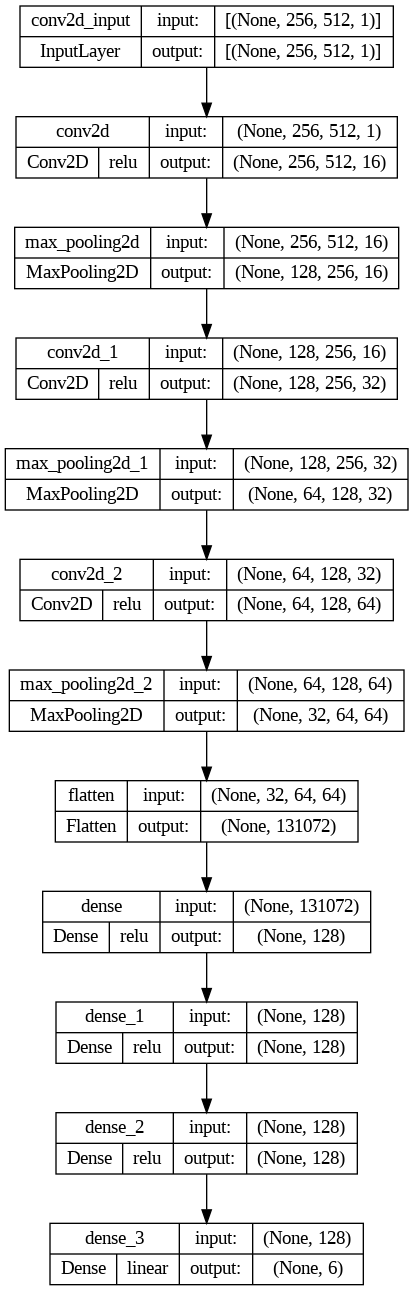
\includegraphics[width= 0.4\textwidth]{img/model_uvwt.png}
        \caption{
                \label{fig:schemat}
                Schemat użytego modelu konwolucyjnego.
        }
\end{figure}
\begin{figure}[H]
        \centering 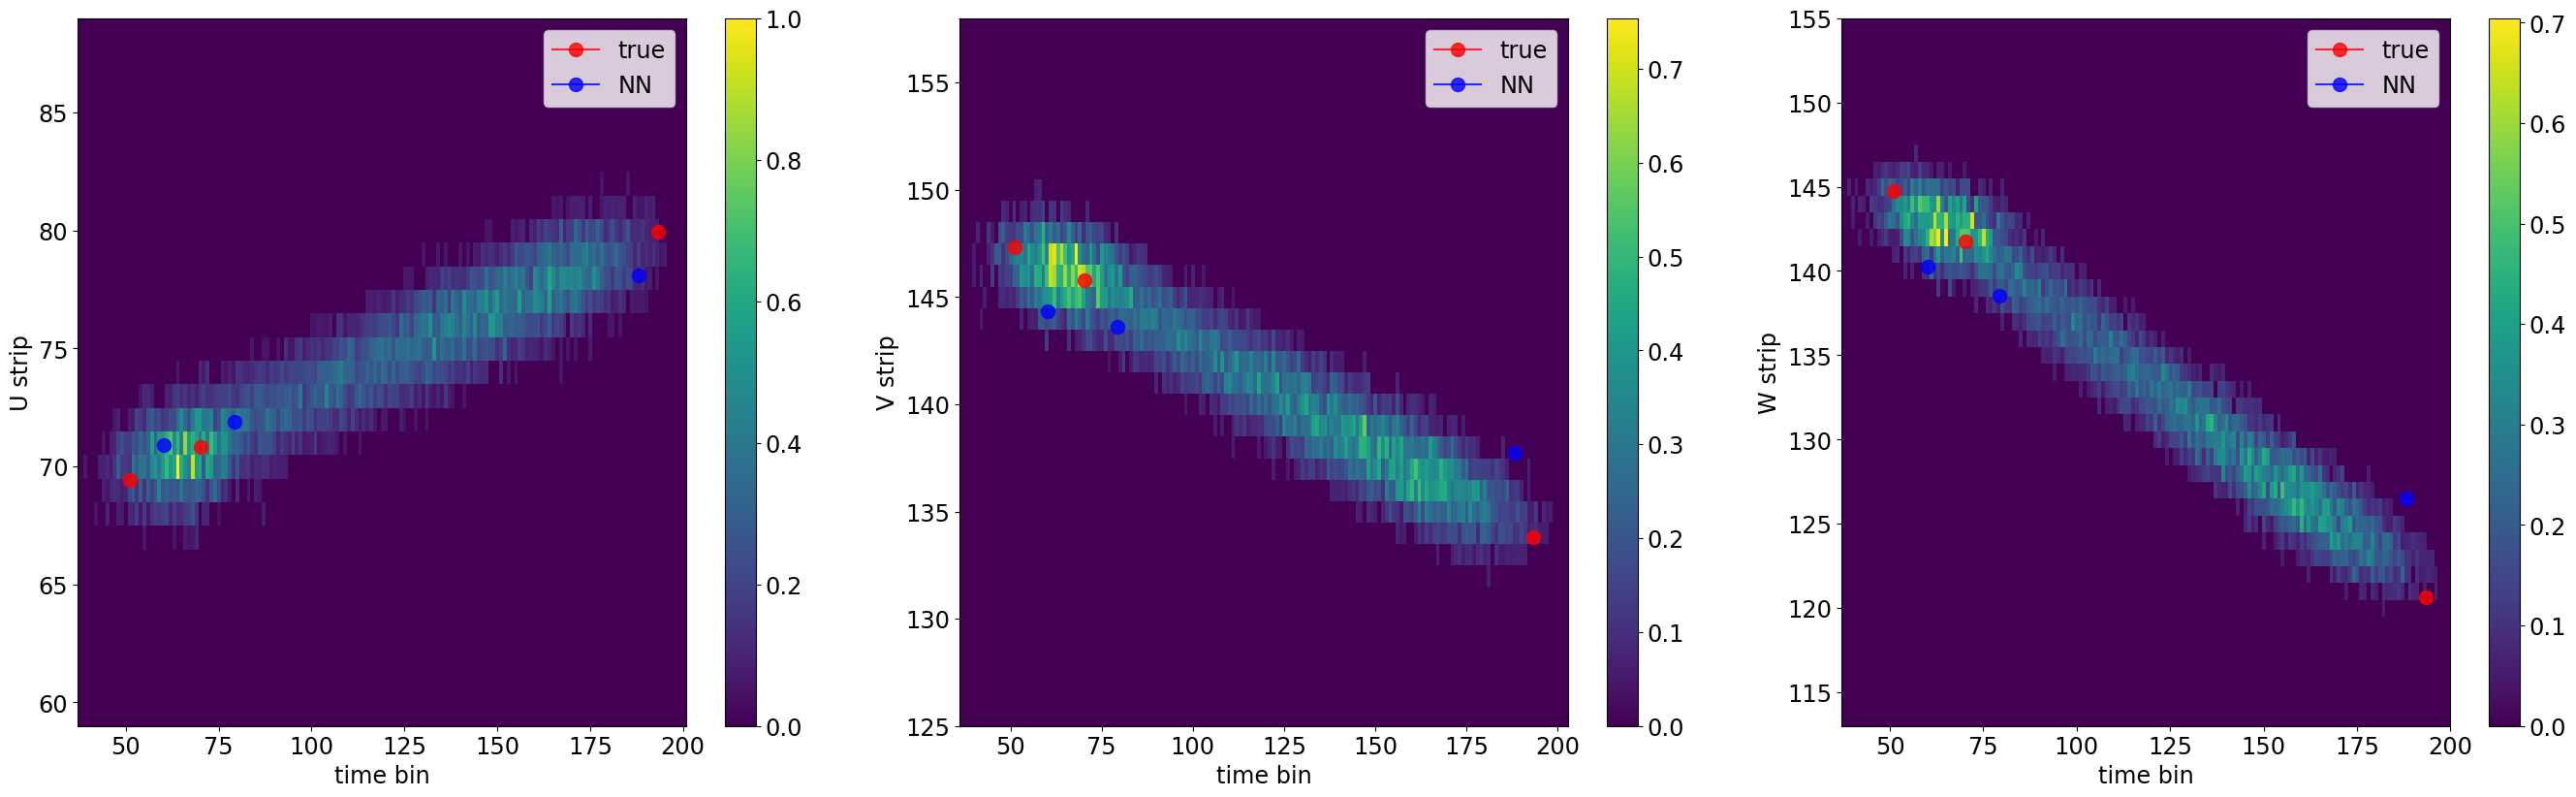
\includegraphics[width= \textwidth]{img/model_uvwt_example.png}
        \caption{
                \label{fig:schemat2}
                Rekonstrukcja położeń punktów uzyskanych w symulacjach (kolor czerwony) przez model (kolor niebieski) dla przykładowego zdarzenia ze zbioru testowego.
        }
\end{figure}

\begin{figure}[H]
    \centering
    \subfloat[\centering ]{{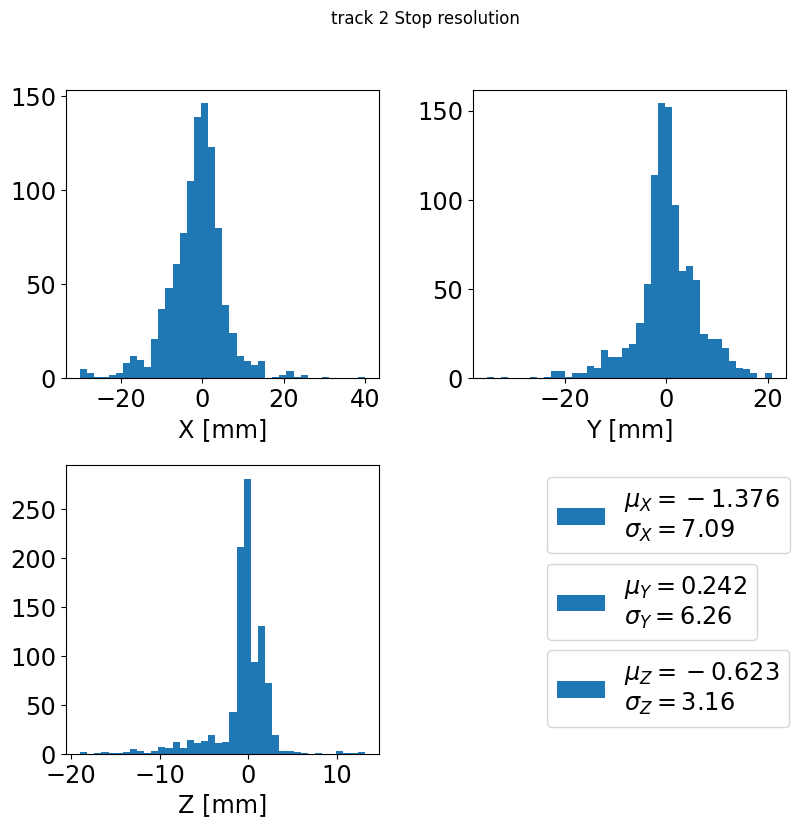
\includegraphics[width=7cm]{img/resultions_1.png} }}
    \qquad
    \subfloat[]{{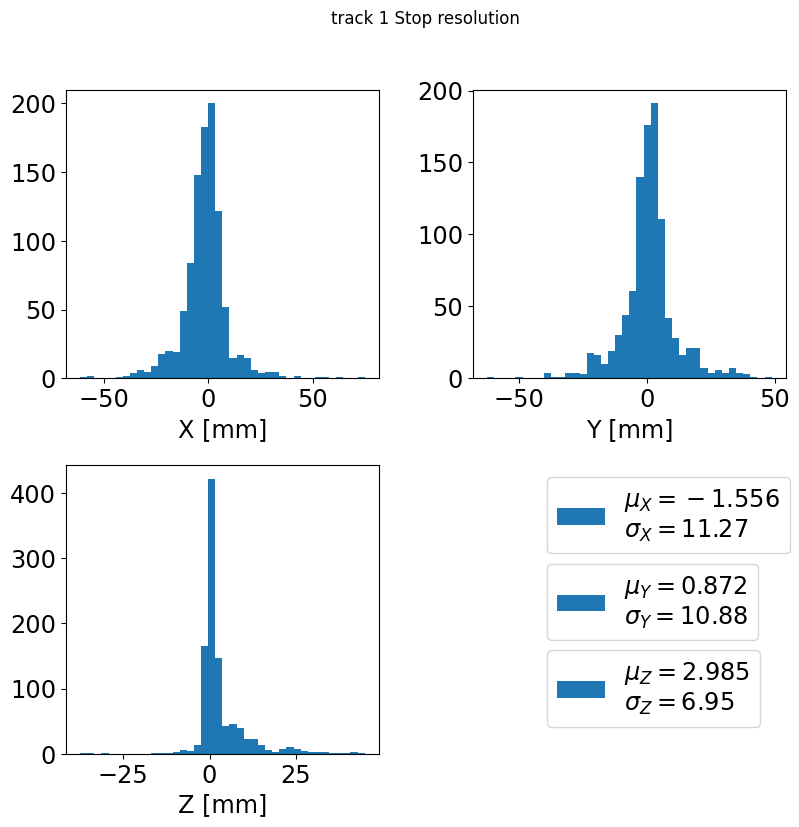
\includegraphics[width=7cm]{img/resolution_2.png} }}
    \qquad
    \subfloat[]{{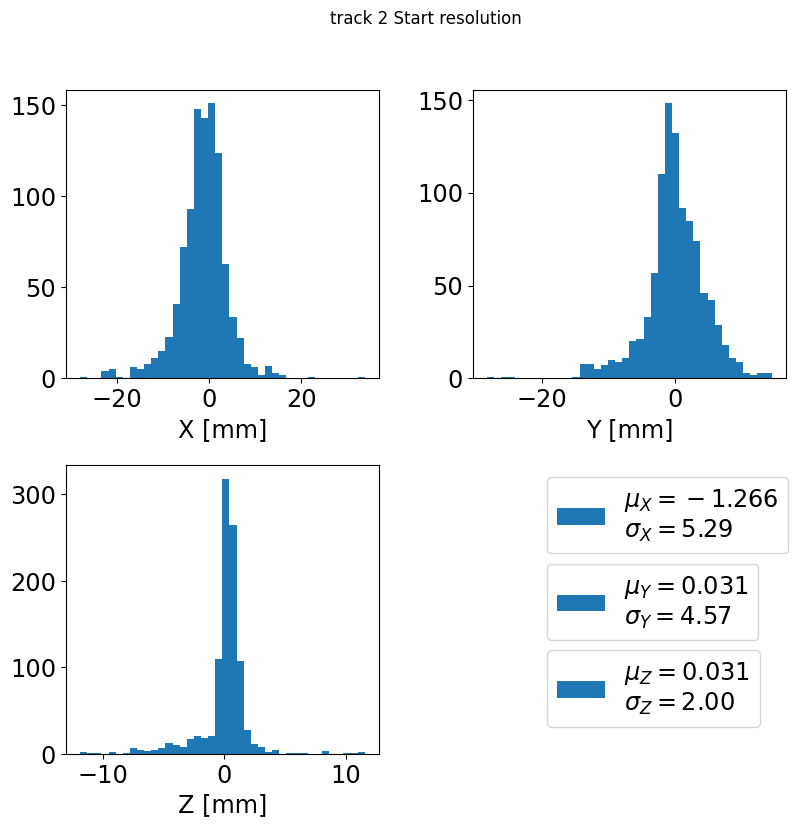
\includegraphics[width=7cm]{img/resolution_3.png} }}
    \caption{Wykresy rozdzielczości współrzędnych punktów w dokonywanej przez model konwolucyjny rekonstrukcji dla przykładów ze zbioru testowego.}
    \label{rys2}
\end{figure}


W \href{https://github.com/mwbaj/MachineLearning/blob/ZPS_2023_winter/WAWTPC/resnet50.ipynb}{\texttt{resnet50.ipynb}} 
znajduje się implementacja modelu ResNet-50, który jednak nie został wytrenowany z racji ograniczeń sprzętowych.\\

% begin{Szymon}
\subsection{Konwersja plików \texttt{.root} na \texttt{.tfrecord}}
W celu przyśpieszenia wczytywania danych przez model napisano program konwertujący pliki \texttt{.root} na \texttt{.tfrecord}.

Program wczytuje mapy ładunku z pliku \texttt{.root}. Następnie, wykorzystując moduł\linebreak \texttt{multiprocessing}, kilka map jednocześnie jest konwertowanych na dane binarne i zapisywanych do oddzielnych plików \texttt{.tfrecord}. Zastosowanie multiprocessingu pozwala znacznie przyśpieszyć proces konwersji. Dodatkową zaletą jest to, że wczytywanie danych w formacie \texttt{.tfrecord} z kilku plików jest szybsze niż z jednego \cite{tfrecord}.

W ramach prostego testu porównano czas wczytania 20 000 zdarzeń z pliku \texttt{.root} i \texttt{.tfrecord}. Wczytywanie danych z pliku \texttt{.root} zajęło 10 min 7 s, a z plików \texttt{.tfrecord} 1 min 9 s, co daje prawie 9-krotne przyśpieszenie. Konwersja z \texttt{.root} na \texttt{.tfrecord} zajęła 8 min 27 s.

Kod oraz demonstracja użycia konwersji \texttt{.root} na \texttt{.tfrecord} dostępny jest w notatniku\linebreak \href{https://github.com/mwbaj/MachineLearning/blob/ZPS_2023_winter/WAWTPC/ROOT_to_TFRecord.ipynb}{\texttt{ROOT\_to\_TFRecord.ipynb}}. Istnieje możliwość zapisania wyjść we współrzędnych XYZ lub UVWT. W notatniku zademonstrowane jest też wczytywanie danych z pliku \texttt{.tfrecord}.
% end{Szymon}

% By Przemysław Szyc - wersja 1.0
\subsection{Dalsze działania}
Sugerowane kolejne działania dotyczące uczenia maszynowego to np:
\begin{enumerate}
    \item Wytrenowanie modelu ResNet-50 w obu formatach danych i porównanie działania modeli;
    \item Poprawa wydajności dotychczasowych modeli poprzez zmianę architektury oraz użycie innego zbioru danych, w szczególności dla rekonstrukcji we współrzędnych UVWT;
    \item Badanie generalizacji modelu do różnych rodzajów danych, w szczególności danych pochodzących z eksperymentu.
\end{enumerate}

% Przemysław Szyc - end

% begin{Szymon}
\section{Konwersja plików \texttt{.graw} na \texttt{.root}}
W ramach prac konserwacyjnych nad repozytorium TPCReco przywrócono do działania program konwertujący pliki \texttt{.graw} na \texttt{EventTPC.root}. Program przystosowano do działania z systemem konfiguracji używającym plików \texttt{.json}, który stosowany jest przez resztę programów w repozytorium.
\subsection{Test \texttt{grawToEventTPC}}
Dodano test \texttt{grawToEventTPC} który:
\begin{enumerate}
    \item testuje poprawność funkcji tworzącej nazwę pliku \texttt{.root}
    \item konwertuje 1 zdarzenie z testowego pliku \texttt{.graw} na \texttt{.root}
    \item sprawdza czy plik \texttt{.root} się otwiera
    \item sprawdza czy ilość zdarzeń jest poprawna
    \item porównuje mapy ładunków załadowane z pliku \texttt{.graw} i \texttt{.root}
    \item sprawdza czy plik \texttt{.root} się zamyka
    \item usuwa plik \texttt{.root}
\end{enumerate}
\subsection{Dalsze kroki}
Kolejnym zadaniem do wykonania w celu usprawnienia rozwijania aplikacji TPCReco może być zastosowanie GitHub Actions~\cite{Actions}. GitHub Actions pozwala na automatyczne wykonanie pewnych czynności w reakcji na zdarzenia dziejące się z repozytorium. Można na przykład automatycznie kompilować aplikację i uruchamiać testy w odpowiedzi na nowy pull request.
\begin{figure}[H]
    \centering
    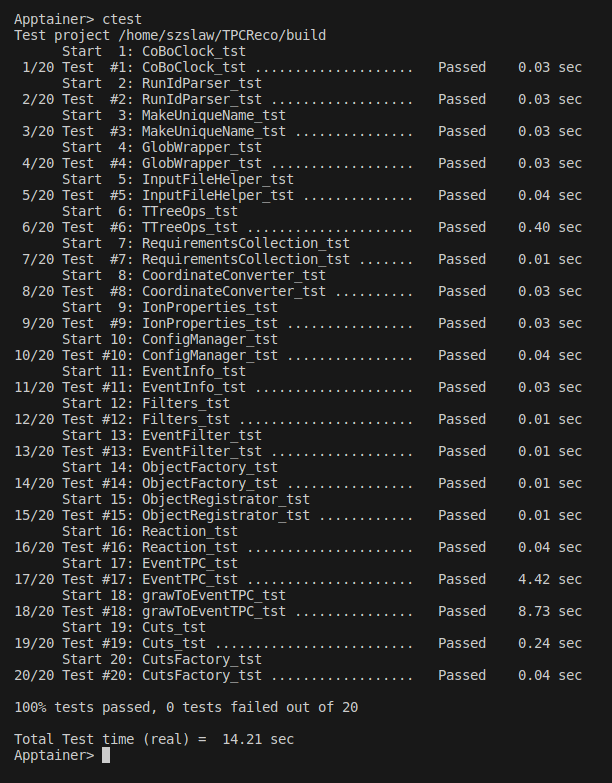
\includegraphics[width=0.5\textwidth]{img/tests.png}
    \caption{Rezultat komendy \texttt{ctest} -- wszystkie testy z wynikiem pozytywnym.}
\end{figure}
% end{Szymon}

\section{Podsumowanie}
% MB
Projekt zespołowy realizowany był w semestrze zimowym roku akademickiego 2023/24 na Wydziale Fizyki Uniwersytetu Warszawskiego. W zakresie celów uzgodnionych z opiekunem projektu, mając na uwadze liczebność zespołu, udało się rozwinąć aplikacje do analizy danych z eksperymentu WarsawTPC zarówno w obszarze przygotowania danych symulowanych i rzeczywistych, jak również usprawnień procesu rekonstrukcji z wykorzystaniem uczenia maszynowego. Zbudowano także bazę wiedzy, która pozwoli na sprawniejsze wprowadzenie nowych uczestników do projektu. 
% /MB

\setcounter{biburllcpenalty}{7}
\setcounter{biburlucpenalty}{8}

\printbibliography[title=Bibliografia]

\end{document}
